\documentclass[12pt]{article}

\usepackage[paper=letterpaper,margin=2.5cm]{geometry} % Set Margins

%% Math and math fonts
\usepackage{amsmath, amsthm, amssymb, amsfonts}
\usepackage{bbold} % for \mathbbm{1}

% date
\usepackage[nodayofweek]{datetime}

% Color
\usepackage{color, xcolor}

% Misc
\usepackage{environ}  % \collect@body in asmmath
\usepackage{graphicx} % \includegraphics options
\usepackage{mdframed} % text boxes
\usepackage{indentfirst} % Indent first paragraph after section header
\usepackage[shortlabels]{enumitem} % Control enumerate items with [(a)]
\usepackage{comment} % Comments
\usepackage{fancyhdr} % Headers and footers

% Tables
\usepackage{array}

% Sub-figures and figure placement
\usepackage{caption}
\usepackage{subcaption}
\usepackage{float} 

% Graphing
\usepackage{pgfplots}
\pgfplotsset{compat=1.17}
\usepackage{tikz}

% Title Placement
\usepackage{titling}
\setlength{\droptitle}{-6em}
\setlength{\headheight}{15pt}

%set indent to 
\setlength{\parindent}{0pt}
\setlength{\parskip}{10pt}

% Hyper refs
\usepackage{hyperref}
\hypersetup{
    colorlinks=true,
    linkcolor=blue,
    urlcolor  = blue,
    filecolor=magenta,      
    urlcolor=blue,
    citecolor = blue,
    anchorcolor = blue
}

% % Citation management
\usepackage{natbib}
\bibliographystyle{abbrvnat}
\setcitestyle{authordate,open={(},close={)}}

% % Move the header up
\usepackage{titling}
%\posttitle{\par\centering}
\preauthor{\centering\normalsize}
\postauthor{\par\centering\vspace{-1em}}
\predate{\centering\normalsize}
\postdate{\par\centering\vspace{-1em}}

% ----------------------------------------
% TITLE
% ----------------------------------------

\pagestyle{fancy}

\lhead{Camacho}
\chead{Class Three}
\rhead{FAME}

\title{FAME Class 4 Notes -- The Math of Environmental Change}
\author{Mariana Camacho}
\date{November 5, 2026}

\begin{document}
\maketitle
\section{Introduction}
\begin{itemize}
    \item New topic for today: derivatives. 
    \item It's okay to carry a sheet with all the rules with you, you just need to know how to use them. 
    \item Mariana will run an optional review and practice session of derivatives next Thursday. 
\end{itemize}

\section{Quick review of modules 1 and 2}
\begin{itemize}
    \item What should come up when we're thinking about systems? Matrices!
    \item Dimensions are important because they tell us whether the matrices are conformable and the size of the result. 
\end{itemize}

\section{The role of derivatives in science}
Science should inform our decisions about the environment. What kind of questions do scientists ask? 
\begin{enumerate}
    \item If I change X, how does Y change?
    \item Is X the same as Y?
\end{enumerate}
Answering both of these questions involves understanding derivatives.

When we ask the first question, we tend to use measurements that might have some incurabilities, and often we will use averages of these. We can also reframe the first question as: how sensitive is Y to changes in X? In environmental management, we often talk about things like climate sensitivity. 

When we hear someone talking about sensitivities, our brain should immediately go to derivatives. 

What kinds of numbers are easier to look at changes with? Real numbers! This is because it's much easier to look at changes when they're smooth than when they're choppy. 

\subsection{Convex and non-convex sets}
Now, let's introduce some notation:\([a,b]\) \& \((a,b)\). 

These are both intervals on the number line. Square brackets \([ ]\) include everything in the interval as well as the upper and lower bounds, while \(( )\) include everything within the interval but not the bounds. 

In \textbf{convex} sets, we can connect any two points without leaving the shape or number line. For \textbf{non-convex} sets we can't do this. 

Here are some examples:

\begin{figure}[H]
    \centering
    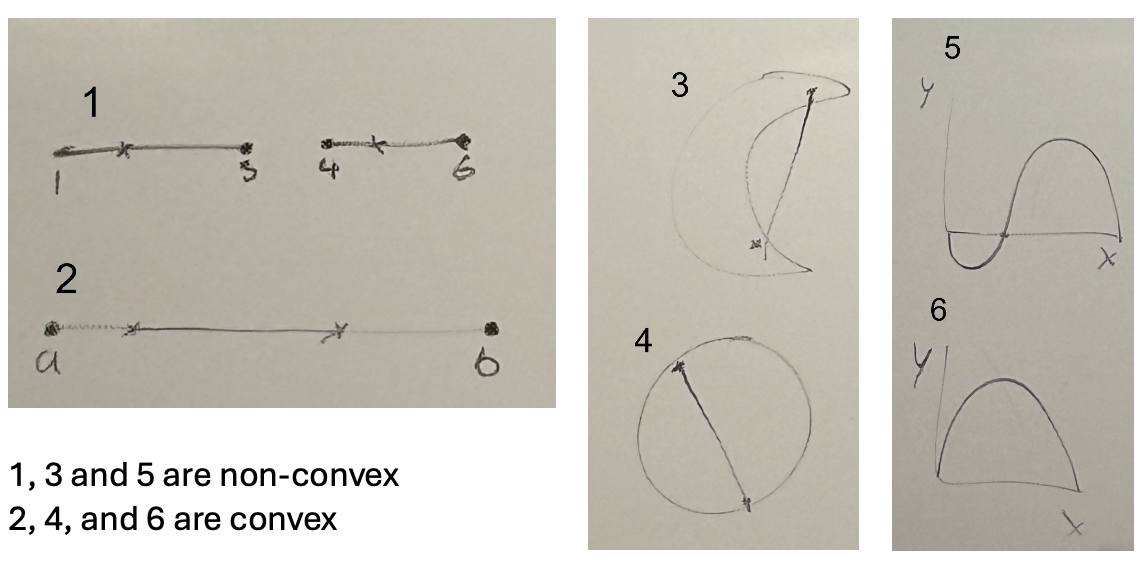
\includegraphics[width=0.75\linewidth]{class_notes/class_4/images/examples.png}
    \label{fig:convex_examples}
\end{figure}

This is important because non-convexities can generate tipping points. In this class, we will mostly work with convex sets, but we have to be careful with non-convex sets because they could lead to irreversibilities (this is a yellow flag). 

More broadly, it's very important to distinguish what results come from the assumptions and which ones come from the data. This is another yellow flag to look out for in the literature.

\subsection{Sequences and series}
A \textbf{sequence} is a list of numbers. We generally think of them as being a result of a function whose domain is the positive integers. 

A \textbf{series} is usually a summation operation on a sequence of numbers. 

Let's look at an example: \([-1,-1/2,-1/3,-1/4,-1/5,...]\)

Here,... means that the sequence keeps going. In these cases, we might worry about the limit: whether the sequence converges to a specific number. In this case, the limit of this sequence is zero. 

A \textbf{monotone} sequence is a sequence that moves in only one direction (it looks like it's tending to the same number).

Now, let's introduce another example: \([-1,1,-1,1,...]\)

This sequence is not monotone, doesn't have a limit, but it is \textbf{bounded} - it doesn't go on to infinity. 

We can define a sequence to be bounded or \textbf{unbounded}. A bounded sequence stays within a specific range (i.e. doesn't go off to infinity). 

The first sequence example would also be bounded. In general, a sequence that has a limit would be bounded. Getting the bounds right can be really important in practice. 

\subsection{Introducing limits}

One of the biggest questions of antiquity was the area of a circle. Now, we know that it's \(\pi r^2\), where \(\pi\) is the ratio from the circumference to the diameter. 

What Archimedes first did was putting a square inside and outside the circle, and taking the average of their areas. Then, he did the same thing with two octagons. He realized that he could keep doing this with any arbitrary number of sides for a polygon. He got up to 64 sides, and got really close to the value of \(\pi\) - close enough for any engineering problem, which is what he was interested in.

\begin{figure}[H]
    \centering
    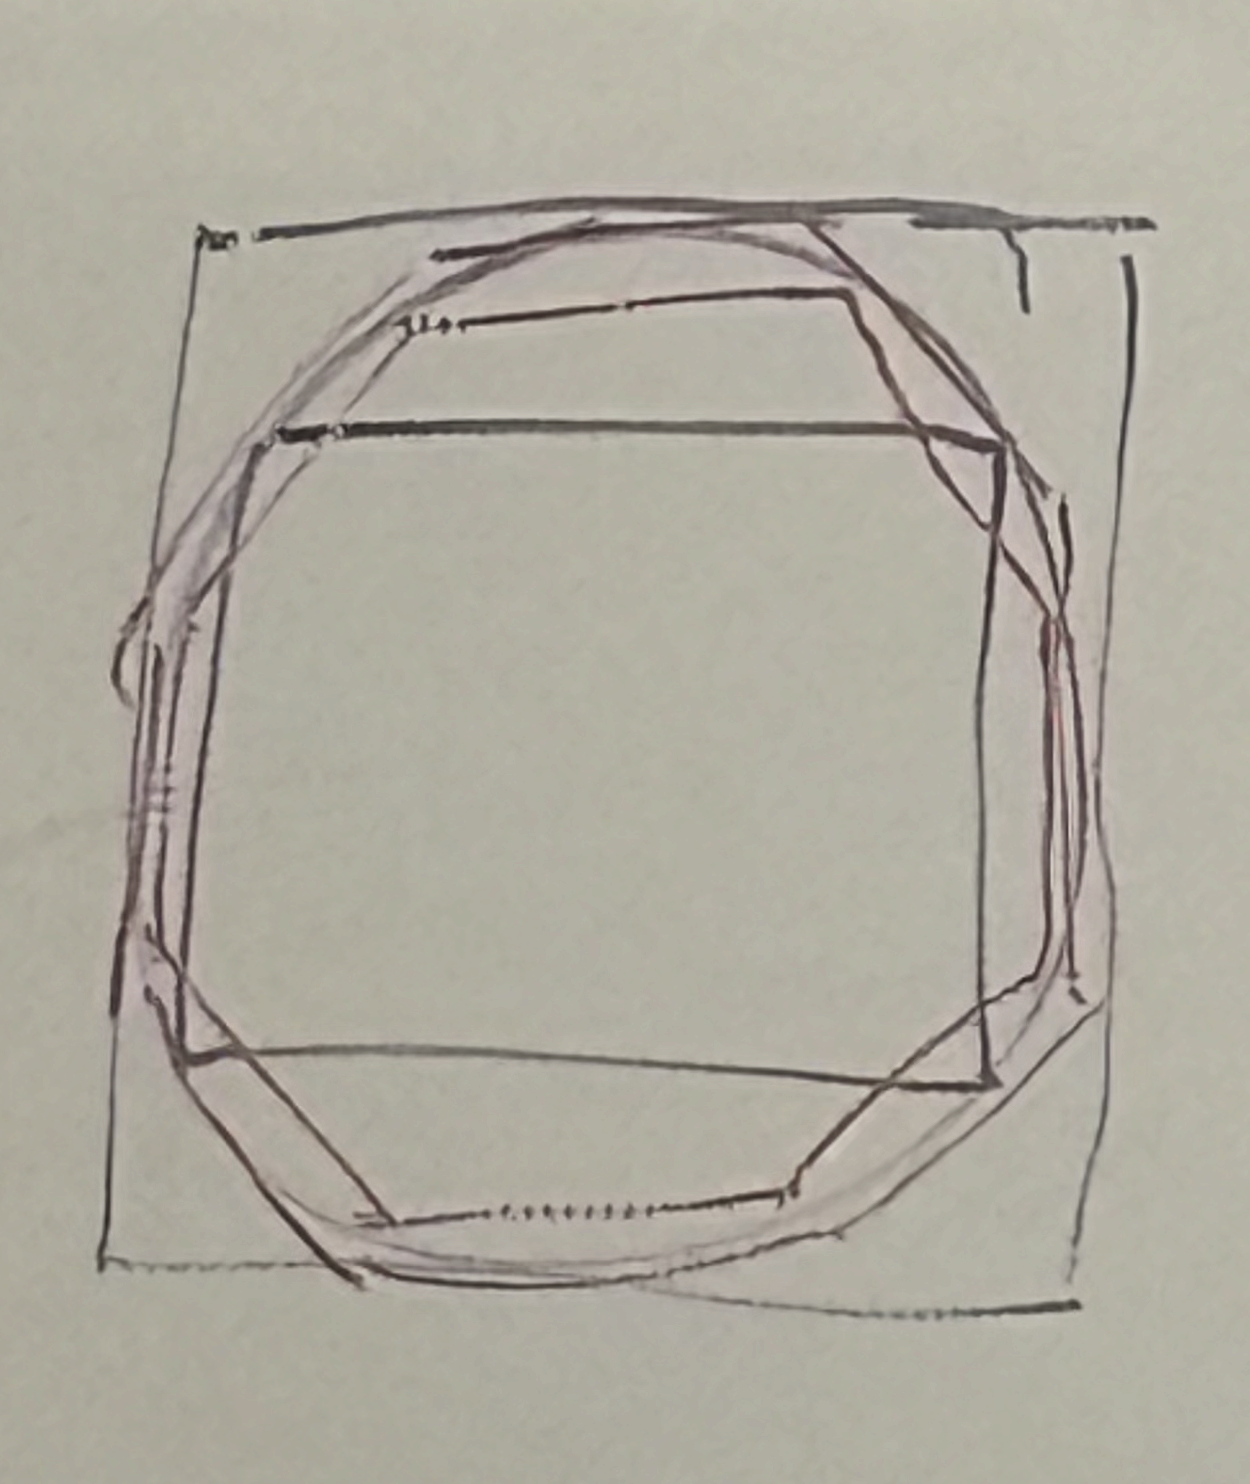
\includegraphics[width=0.25\linewidth]{class_notes/class_4/images/archimedes.png}
    \label{fig:archimedes}
\end{figure}

He came really close to discovering calculus, centuries before Newton and Leibniz. What he was missing was adding the \(\ ...\), taking the limit, which was very taboo in ancient Greece. 

We can think of \textbf{infinity} of the process of continuing on. Now, let's look at some examples of limits.

\[
\lim_{\substack{N \to 0 \\ a > 0}} \frac{a}{N} = \infty
\]
\[
\lim_{\substack{N \to \infty \\ 0 < a < \infty}} \frac{N}{N+a} = 1
\]

Let's look at a more interesting example:

\[
\lim_{\substack{N \to \infty}} \left(1+\frac{1}{N}\right)^N = ?
\]

If we start plugging in the numbers, we will find that:

\[
\begin{array}{c|c|c}
N & \text{Calculation} & \text{Value} \\
\hline
1 & (1+1)^1 & 2.0000 \\
2 & (1+1/2)^2 & 2.2500 \\
3 & (1+1/3)^3 & 2.3704
\end{array}
\]

If we keep doing this, we will find that:
\[
\lim_{\substack{N \to \infty}} \left(1+\frac{1}{N}\right)^N = e \approx 2.71828
\]

Limits are fundamental to the sustainability conversation, because they allow us to compare different infinite processes. 

\subsection{Intermediate value theorem and derivatives}

We can think of the secant line as a good approximation for the function between two points. We can do better by picking an intermediate value and making a new secant line. This is the key idea of the \textbf{intermediate value theorem}. The key idea is that we get a better localized measurement by taking two values closer together.

\begin{figure}[H]
    \centering
    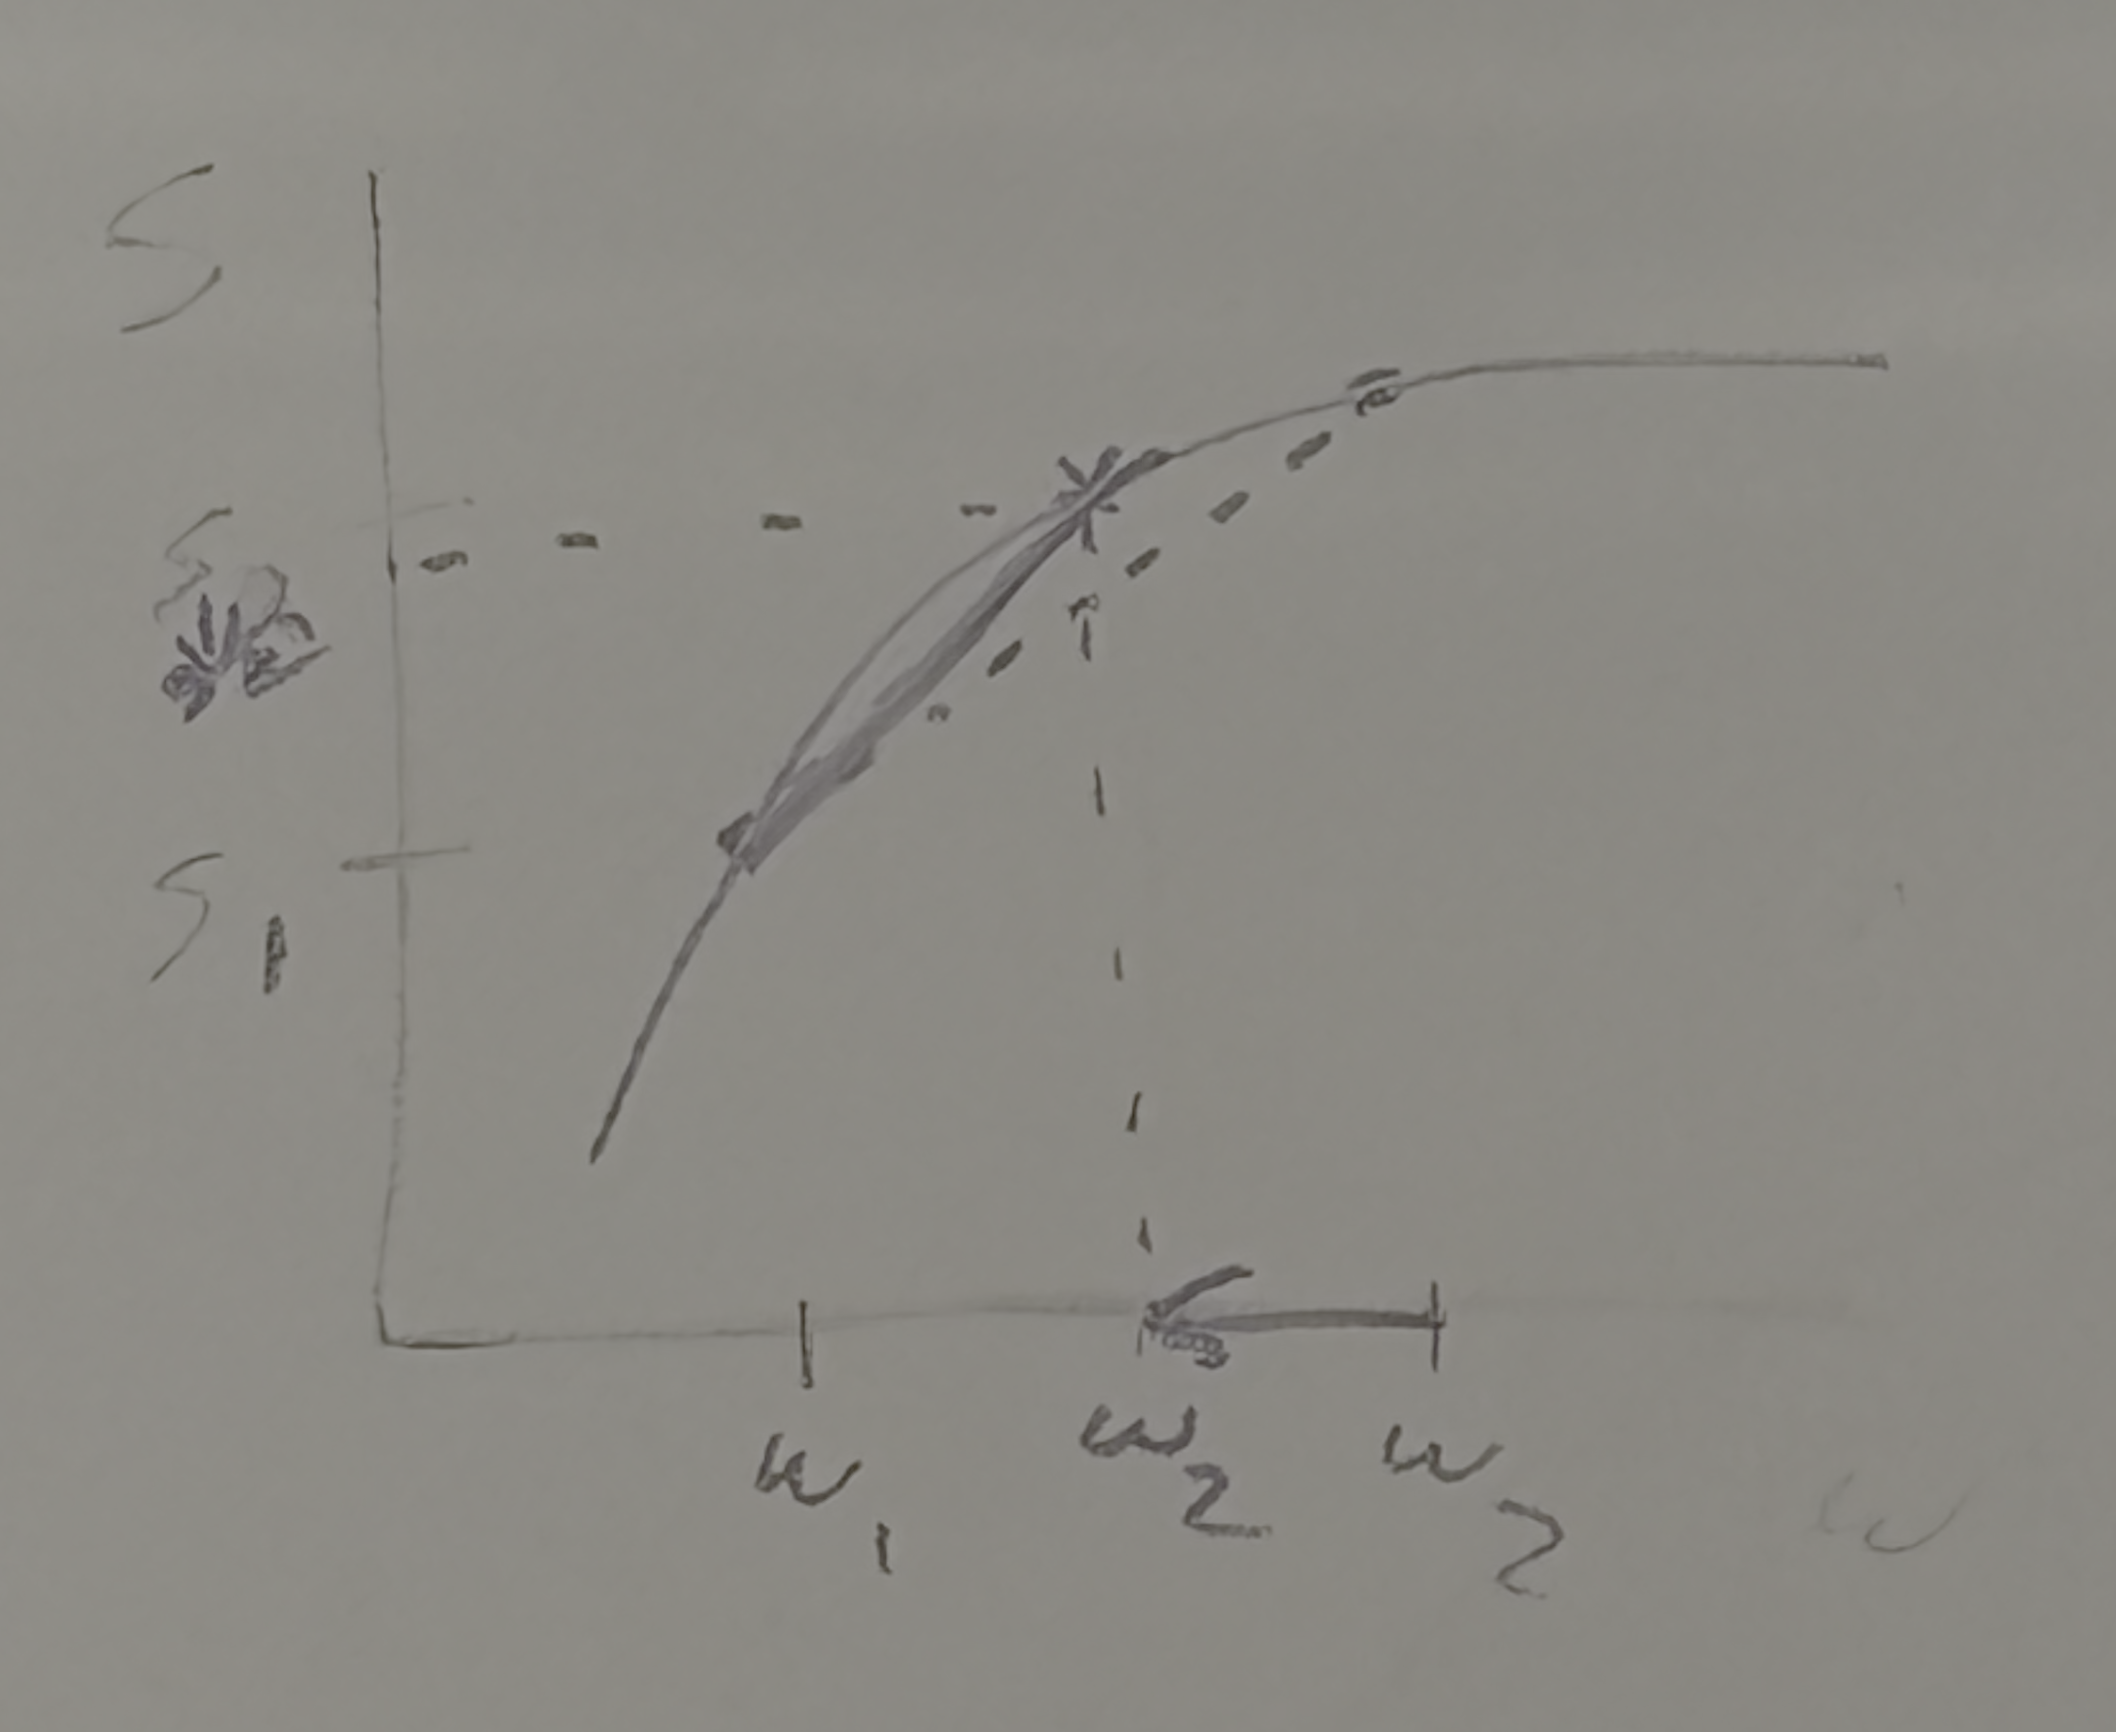
\includegraphics[width=0.5\linewidth]{class_notes/class_4/images/IVT.png}
    \label{fig:IVT}
\end{figure}

This leads us to a formal expression:

\[
\frac{ \Delta s}{\Delta w} = \frac{f(w_2)-f(w_1)}{w_2-w_1}
\]

What we tend to do with this expression, is moving \(w_2\) and \(w_1\) closer and closer together, so that:

\[
  \frac{ds}{dw} = \lim_{\epsilon \to 0} \frac{f(w_1+G)-f(w1)}{\epsilon} 
\]

This is the formal definition of a \textbf{derivative}. 

We can also define the derivative as the rise over the run in a plot. 
\begin{figure}[H]
    \centering
    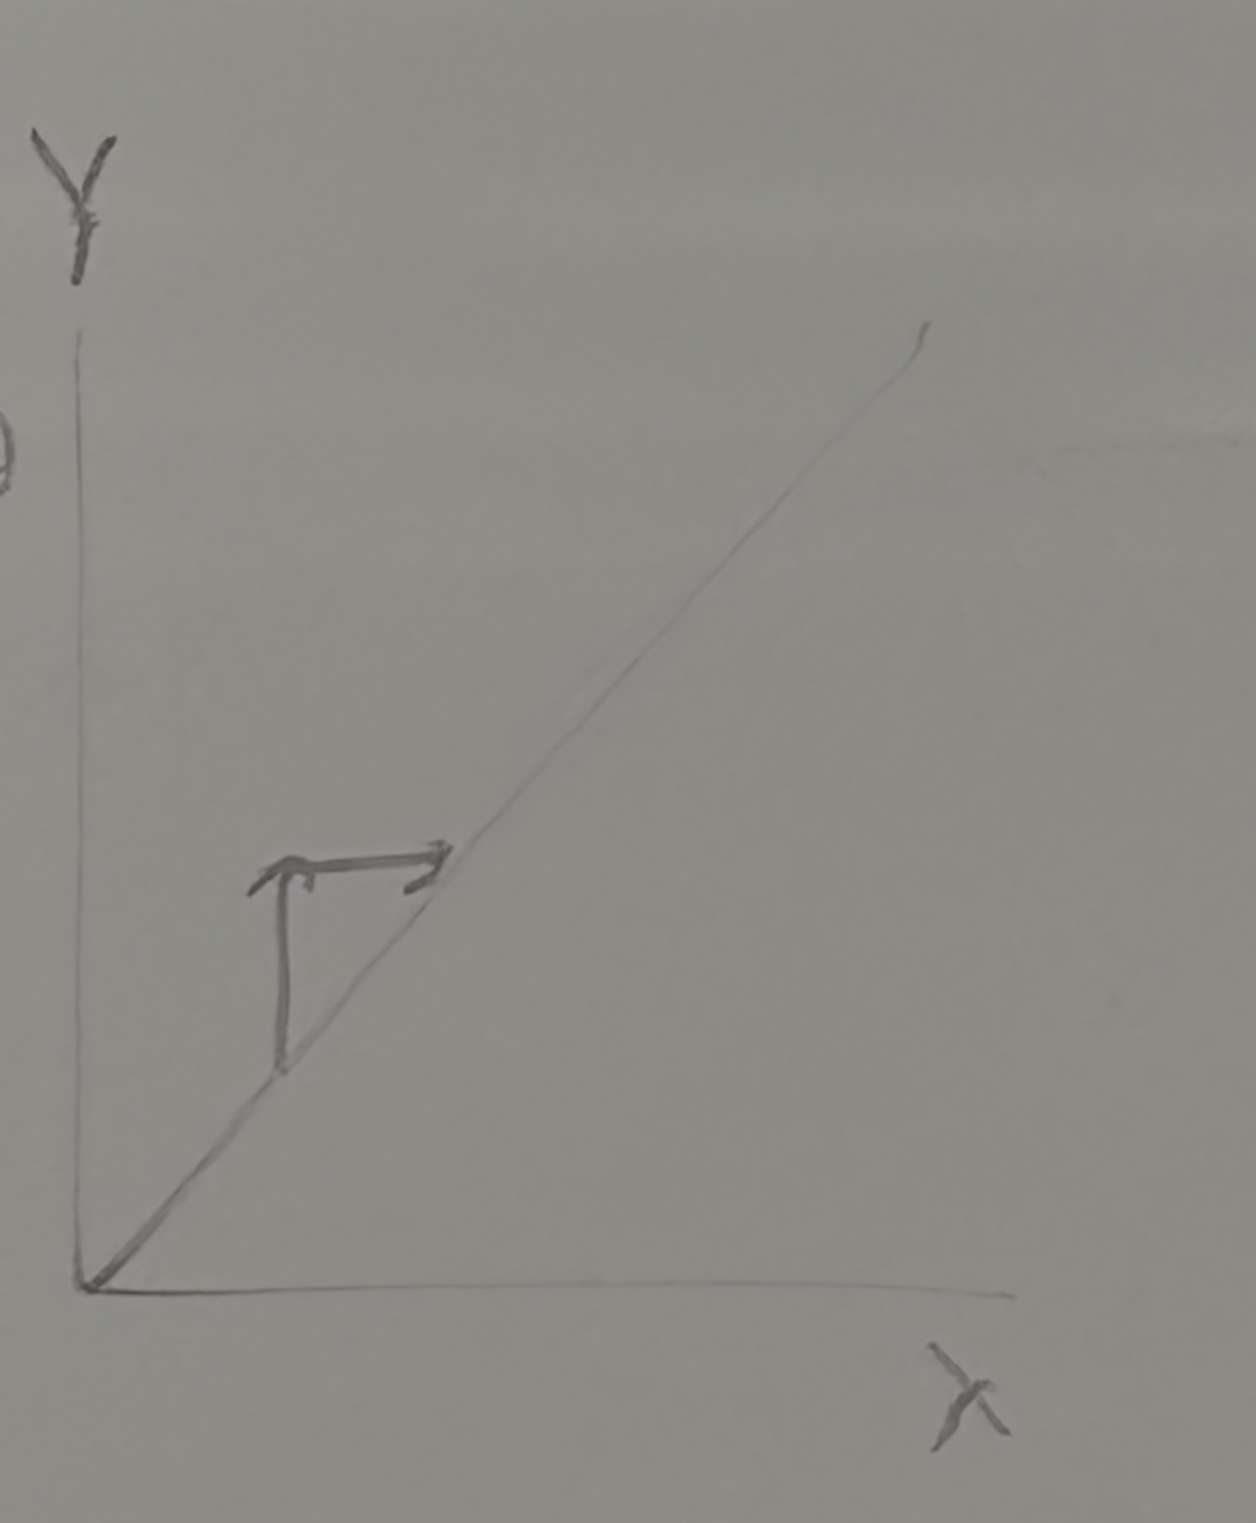
\includegraphics[width=0.25\linewidth]{class_notes/class_4/images/plot.png}
    \label{fig:plot}
\end{figure}

Let's look at this another way:

\[
\begin{aligned}
w &= x \\
f(x) &= ax \\[6pt]
f'(x) &= \lim_{\epsilon \to 0}
\frac{f(x+\epsilon)-f(x)}{\epsilon} \\[6pt]
&= \lim_{\epsilon \to 0}
\frac{a(x+\epsilon)-ax}{\epsilon} \\[6pt]
&= \lim_{\epsilon \to 0}
\frac{ax+a\epsilon-ax}{\epsilon} \\[6pt]
&= \lim_{\epsilon \to 0}
\frac{a\epsilon}{\epsilon} \\[6pt]
&= a
\end{aligned}
\]


\end{document}